\documentclass[border=3pt]{standalone}
% Preâmbulo compartilhado pelos diagramas TikZ da aula 5 de IHC (Processos de Design)
\usepackage[T1]{fontenc}
\usepackage[utf8]{inputenc}
\usepackage{lmodern}
\usepackage{amsmath}
\usepackage{xcolor}
\usepackage{tikz}
\usetikzlibrary{arrows.meta,angles,quotes,decorations.pathmorphing,calc,
                positioning,shapes.geometric,shapes.misc,backgrounds,fit,
                math}

% Paleta (mesma dos SVGs originais)
% Paleta da disciplina de IHC: acento roxo (#755099), da capa do livro.
% (o nome "dblue" é mantido para não alterar todos os diagramas)
\definecolor{dblue}{HTML}{755099}
\definecolor{dorange}{HTML}{B3541E}
\definecolor{dgreen}{HTML}{4A7C59}
\definecolor{dred}{HTML}{9C4B4B}
\definecolor{dcream}{HTML}{F4F1EA}
\definecolor{dshade}{HTML}{DDD7C9}

% Função gaussiana (não normalizada por padrão de escala visual)
\pgfmathdeclarefunction{gauss}{3}{%
  \pgfmathparse{1/(#3*sqrt(2*pi))*exp(-((#1-#2)^2)/(2*#3^2))}%
}

% Estilos comuns (prefixo d... para não colidir com chaves internas do pgf)
\tikzset{
  >={Stealth[length=2mm]},
  dguide/.style={gray!55, dashed, line width=0.4pt},
  daxis/.style={gray!60, line width=0.7pt, ->},
  dbody/.style={fill=black!3, draw=black!80, line width=1pt},
  dacc/.style={draw=dblue, line width=1pt},
  dlbl/.style={black!55, font=\small},
  dsub/.style={black!45, font=\footnotesize},
  dstate/.style={circle, draw=black!80, fill=dcream, line width=1pt,
                 minimum size=17mm, font=\large, inner sep=1pt},
  dobs/.style={circle, draw=black!80, fill=dshade, line width=1pt,
               minimum size=14mm, font=\large, inner sep=1pt},
  dbox/.style={rounded corners=2pt, draw=black!80, fill=dcream, line width=1pt,
               align=center, inner sep=6pt},
  dop/.style={circle, draw=black!80, fill=white, line width=1pt,
              minimum size=6mm, inner sep=0pt, font=\small},
  dtrans/.style={->, dblue, line width=1pt},
  dmeas/.style={->, dorange, line width=1pt},
  dcurve/.style={line width=1pt, dblue},
  dcurveb/.style={line width=1.4pt, dorange},
}

\begin{document}
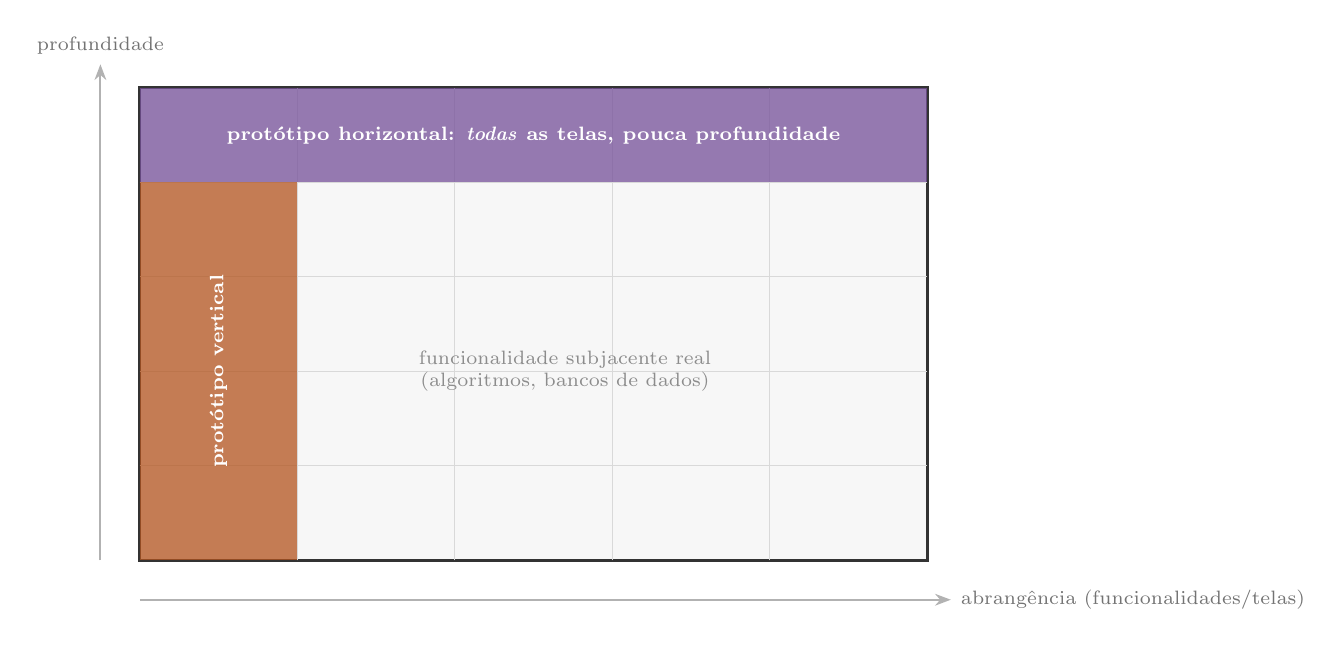
\begin{tikzpicture}[x=1cm,y=1cm]

  \draw[dbody, line width=1.1pt] (0,0) rectangle (10,6);
  \foreach \x in {2,4,6,8} { \draw[black!15, line width=0.4pt] (\x,0) -- (\x,6); }
  \foreach \y in {1.2,2.4,3.6,4.8} { \draw[black!15, line width=0.4pt] (0,\y) -- (10,\y); }

  % protótipo horizontal: faixa fina cobrindo todas as funcionalidades
  \fill[dblue, opacity=0.75] (0,4.8) rectangle (10,6);
  \node[white, font=\scriptsize\bfseries] at (5,5.4) {protótipo horizontal: \textit{todas} as telas, pouca profundidade};

  % protótipo vertical: coluna estreita, toda a profundidade
  \fill[dorange, opacity=0.75] (0,0) rectangle (2,4.8);
  \node[white, font=\scriptsize\bfseries, rotate=90] at (1,2.4) {protótipo vertical};

  \draw[daxis] (0,-0.5) -- (10.3,-0.5) node[right, dlbl, font=\scriptsize] {abrangência (funcionalidades/telas)};
  \draw[daxis] (-0.5,0) -- (-0.5,6.3) node[above, dlbl, font=\scriptsize] {profundidade};

  \node[dsub, font=\scriptsize, align=center, text width=9cm] at (5.4,2.4) {funcionalidade subjacente real\\(algoritmos, bancos de dados)};


\end{tikzpicture}
\end{document}
